\graphicspath{{./images/}}

\newgeometry{left=2.5cm, right=2.5cm, bottom=2.5cm, top=2.5cm}

\begin{landscape}
	
\chapter{Projektmanagement}

Obschon ein iteratives Vorgehen wie Scrum als Methode für die Erarbeitung der Masterthesis verwendet wird, ist es für den Überblick der Arbeit unumgänglich eine groben Projektplan vorliegen zu haben. Neben dem Plan wurden auch allfällige Risiken und die damit verbundenen Massnahmen aufgelistet. Diese beziehen sich auf Risiken für die Umsetzung der Thesis und des Umfeldes. Im Software Architektur Dokument Im Kapitel 11 sind die technischen Risiken der Architektur aufgeführt.


\section{Projektplan}

Der Projektplan wurde grob gehalten und nur die wichtigsten Aufgaben aufgenommen um den Plan nicht zu überladen. Die Reserve am Schluss dient als Puffer falls sich trotz der Planung Probleme ergeben sollten.

\begin{center}
	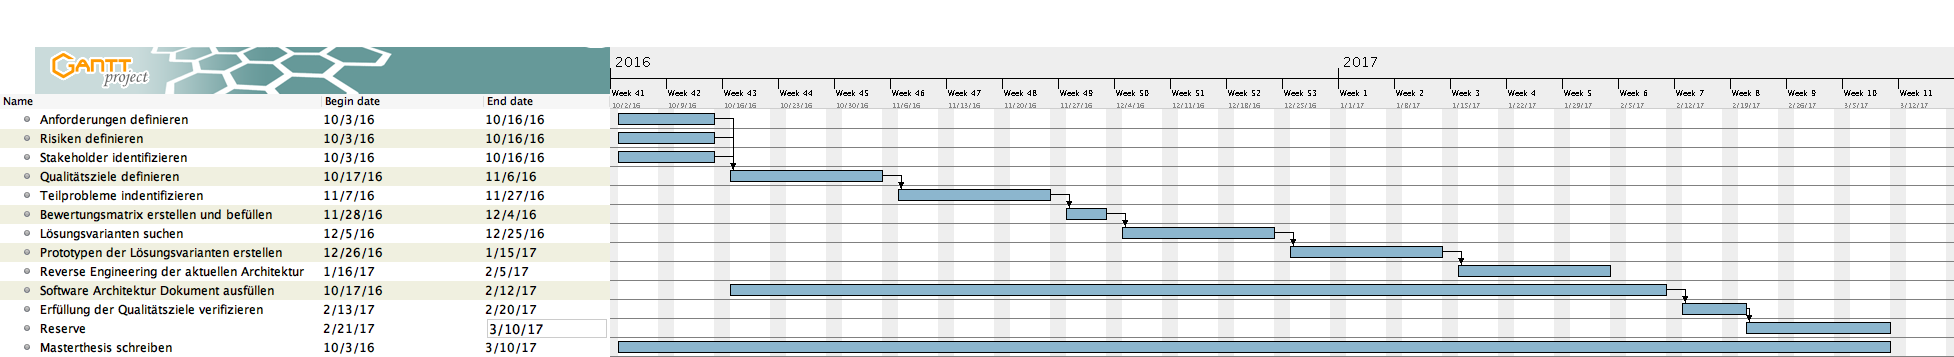
\includegraphics[scale=0.37]{projectplan.png}
\end{center}
\newpage	

\section{Risiken}
\begin{table}[h!]
	\centering
	\caption{Risiken}
	\begin{tabular}{ | p{2cm} | p{10cm} | p{10cm} | }
		\toprule
		{\textbf{Risiko}} & {\textbf{Beschreibung}} & {\textbf{Massnahmen}} \\
		\midrule
		Richtlininen der Firma & Abklärungen und Vorschläge wie die Richtlinien eingehalten werden können oder angepasst werden müssten. & Die bestehenden Richtlinien werden von der Applikation bereits eingehalten. Die Vorgaben bezüglich Change Management müssen frühzeitig angegangen werden da es Einfluss auf den Prozess hat. \\ \hline
		Conway's law & Conway's law ist eine Beziehung zwischen der Firmenorganisation und der Softwarearchitektur. Das Gesetz besagt, dass die Software Architektur eines Systems sich nach der Firma richtet. & Obschon die Organisation noch eher klassisch aufgebaut ist, sind durch firmeninterne Initiativen die Entwicklungsabteilungen nicht so stark an Vorgaben gebunden. Dennoch ist das Risiko im Auge zu behalten. \\ \hline
		Fehlende Requirements & Das Projekt wurde in kurzer Zeit umgesetzt und hat deshalb keinen formalen Requirement Engineering Prozess durchlaufen. Dadurch sind weder funktionale noch nicht funktionalen Anforderungsdokumente vorhanden. & Die Requirements nach zu erfassen ist in diesem Fall nicht zielführend, da es nur einen hohen Aufwand ohne Mehrwert verursacht. Da die Applikation überschaubar ist und einen klaren Business Case hat,  wird dieser im Software Architektur Dokument beschrieben.\\ \hline
		Neue Requirements & Die Requirements für die Architekturanpassung sind nicht definiert. & Da die Anforderung von der Entwicklungsabteilung getrieben wird, sollen die Basisanforderungen als erstes erfasst werden. Änderungen oder Ergänzungen sollen nach-dokumentiert werden.\\
		\bottomrule
	\end{tabular}
\end{table}

\end{landscape}
\restoregeometry